\documentclass[12pt]{article}\usepackage[]{graphicx}\usepackage[]{color}
%% maxwidth is the original width if it is less than linewidth
%% otherwise use linewidth (to make sure the graphics do not exceed the margin)
\makeatletter
\def\maxwidth{ %
  \ifdim\Gin@nat@width>\linewidth
    \linewidth
  \else
    \Gin@nat@width
  \fi
}
\makeatother

\definecolor{fgcolor}{rgb}{0.345, 0.345, 0.345}
\newcommand{\hlnum}[1]{\textcolor[rgb]{0.686,0.059,0.569}{#1}}%
\newcommand{\hlstr}[1]{\textcolor[rgb]{0.192,0.494,0.8}{#1}}%
\newcommand{\hlcom}[1]{\textcolor[rgb]{0.678,0.584,0.686}{\textit{#1}}}%
\newcommand{\hlopt}[1]{\textcolor[rgb]{0,0,0}{#1}}%
\newcommand{\hlstd}[1]{\textcolor[rgb]{0.345,0.345,0.345}{#1}}%
\newcommand{\hlkwa}[1]{\textcolor[rgb]{0.161,0.373,0.58}{\textbf{#1}}}%
\newcommand{\hlkwb}[1]{\textcolor[rgb]{0.69,0.353,0.396}{#1}}%
\newcommand{\hlkwc}[1]{\textcolor[rgb]{0.333,0.667,0.333}{#1}}%
\newcommand{\hlkwd}[1]{\textcolor[rgb]{0.737,0.353,0.396}{\textbf{#1}}}%
\let\hlipl\hlkwb

\usepackage{framed}
\makeatletter
\newenvironment{kframe}{%
 \def\at@end@of@kframe{}%
 \ifinner\ifhmode%
  \def\at@end@of@kframe{\end{minipage}}%
  \begin{minipage}{\columnwidth}%
 \fi\fi%
 \def\FrameCommand##1{\hskip\@totalleftmargin \hskip-\fboxsep
 \colorbox{shadecolor}{##1}\hskip-\fboxsep
     % There is no \\@totalrightmargin, so:
     \hskip-\linewidth \hskip-\@totalleftmargin \hskip\columnwidth}%
 \MakeFramed {\advance\hsize-\width
   \@totalleftmargin\z@ \linewidth\hsize
   \@setminipage}}%
 {\par\unskip\endMakeFramed%
 \at@end@of@kframe}
\makeatother

\definecolor{shadecolor}{rgb}{.97, .97, .97}
\definecolor{messagecolor}{rgb}{0, 0, 0}
\definecolor{warningcolor}{rgb}{1, 0, 1}
\definecolor{errorcolor}{rgb}{1, 0, 0}
\newenvironment{knitrout}{}{} % an empty environment to be redefined in TeX

\usepackage{alltt}
\usepackage{amsmath}
\usepackage{amssymb}
\usepackage{graphicx}
\usepackage{fullpage}
\usepackage{setspace}
\usepackage{hyperref}
\usepackage{color}
\onehalfspacing
\IfFileExists{upquote.sty}{\usepackage{upquote}}{}
\begin{document}

\title{Pol Sci 630: Problem Set 8 - Data Management and Omitted Variable Bias - Solutions}

\author{Prepared by: Jan Vogler (\href{mailto:jan.vogler@duke.edu}{jan.vogler@duke.edu})}

\date{Grading Due Date: Friday, October 28th, 1.40 PM (Beginning of Lab)}
 
\maketitle



\textbf{\color{red} Insert your comments on the assignment that you are grading above the solution in bold and red text. For example write: ``GRADER COMMENT: everything is correct!" Also briefly point out which, if any, problems were not solved correctly and what the mistake was. See below for more examples.}

\bigskip

\textbf{In order to make your text bold and red, you need to insert the following line at the beginning of the document:}

\begin{verbatim} \usepackage{color} \end{verbatim}

\textbf{and the following lines above the solution of the specific task:}

\begin{verbatim} \textbf{\color{red} GRADER COMMENT: everything is correct!} \end{verbatim}



\pagebreak

\section*{R Programming}

\subsection*{Problem 1}

\begin{knitrout}
\definecolor{shadecolor}{rgb}{0.969, 0.969, 0.969}\color{fgcolor}\begin{kframe}
\begin{alltt}
\hlcom{### a}

\hlkwd{setwd}\hlstd{(}\hlstr{"C:/Users/Jan/OneDrive/Documents/GitHub/ps630_lab/ps630_f16/W8"}\hlstd{)}

\hlkwd{library}\hlstd{(foreign)}

\hlstd{vote1} \hlkwb{=} \hlkwd{read.dta}\hlstd{(}\hlstr{"VOTE1.dta"}\hlstd{)}

\hlstd{vote1}\hlopt{$}\hlstd{expendA_sq} \hlkwb{=} \hlstd{(vote1}\hlopt{$}\hlstd{expendA)}\hlopt{^}\hlnum{2}

\hlkwd{summary}\hlstd{(vote1)}
\end{alltt}
\begin{verbatim}
##     state              district          democA           voteA     
##  Length:173         Min.   : 1.000   Min.   :0.0000   Min.   :16.0  
##  Class :character   1st Qu.: 3.000   1st Qu.:0.0000   1st Qu.:36.0  
##  Mode  :character   Median : 6.000   Median :1.0000   Median :50.0  
##                     Mean   : 8.838   Mean   :0.5549   Mean   :50.5  
##                     3rd Qu.:11.000   3rd Qu.:1.0000   3rd Qu.:65.0  
##                     Max.   :42.000   Max.   :1.0000   Max.   :84.0  
##     expendA            expendB           prtystrA        lexpendA     
##  Min.   :   0.302   Min.   :   0.93   Min.   :22.00   Min.   :-1.197  
##  1st Qu.:  81.634   1st Qu.:  60.05   1st Qu.:44.00   1st Qu.: 4.402  
##  Median : 242.782   Median : 221.53   Median :50.00   Median : 5.492  
##  Mean   : 310.611   Mean   : 305.09   Mean   :49.76   Mean   : 5.026  
##  3rd Qu.: 457.410   3rd Qu.: 450.72   3rd Qu.:56.00   3rd Qu.: 6.126  
##  Max.   :1470.674   Max.   :1548.19   Max.   :71.00   Max.   : 7.293  
##     lexpendB            shareA           expendA_sq       
##  Min.   :-0.07257   Min.   : 0.09464   Min.   :      0.1  
##  1st Qu.: 4.09524   1st Qu.:18.86800   1st Qu.:   6664.1  
##  Median : 5.40056   Median :50.84990   Median :  58943.1  
##  Mean   : 4.94437   Mean   :51.07654   Mean   : 174975.6  
##  3rd Qu.: 6.11084   3rd Qu.:84.25510   3rd Qu.: 209223.9  
##  Max.   : 7.34484   Max.   :99.49500   Max.   :2162881.9
\end{verbatim}
\begin{alltt}
\hlstd{lm_vote_curv} \hlkwb{=} \hlkwd{lm}\hlstd{(voteA} \hlopt{~} \hlstd{expendA} \hlopt{+} \hlstd{expendA_sq} \hlopt{+} \hlstd{expendB} \hlopt{+} \hlstd{prtystrA,} \hlkwc{data} \hlstd{= vote1)}

\hlkwd{summary}\hlstd{(lm_vote_curv)}
\end{alltt}
\begin{verbatim}
## 
## Call:
## lm(formula = voteA ~ expendA + expendA_sq + expendB + prtystrA, 
##     data = vote1)
## 
## Residuals:
##     Min      1Q  Median      3Q     Max 
## -24.286  -7.101  -1.368   7.340  29.620 
## 
## Coefficients:
##               Estimate Std. Error t value Pr(>|t|)    
## (Intercept)  2.822e+01  4.083e+00   6.912 9.51e-11 ***
## expendA      7.159e-02  6.683e-03  10.713  < 2e-16 ***
## expendA_sq  -3.854e-05  6.249e-06  -6.167 5.01e-09 ***
## expendB     -3.051e-02  2.811e-03 -10.857  < 2e-16 ***
## prtystrA     3.235e-01  7.972e-02   4.059 7.55e-05 ***
## ---
## Signif. codes:  0 '***' 0.001 '**' 0.01 '*' 0.05 '.' 0.1 ' ' 1
## 
## Residual standard error: 10.07 on 168 degrees of freedom
## Multiple R-squared:  0.6483,	Adjusted R-squared:  0.6399 
## F-statistic: 77.41 on 4 and 168 DF,  p-value: < 2.2e-16
\end{verbatim}
\begin{alltt}
\hlcom{### b}

\hlstd{nd} \hlkwb{=} \hlkwd{data.frame}\hlstd{(}\hlkwc{expendA} \hlstd{=} \hlkwd{seq}\hlstd{(}\hlkwd{min}\hlstd{(vote1}\hlopt{$}\hlstd{expendA),} \hlkwd{max}\hlstd{(vote1}\hlopt{$}\hlstd{expendA),} \hlkwc{length.out} \hlstd{=} \hlnum{11}\hlstd{),}
    \hlkwc{expendB} \hlstd{=} \hlkwd{rep}\hlstd{(}\hlkwd{mean}\hlstd{(vote1}\hlopt{$}\hlstd{expendB),} \hlnum{11}\hlstd{),} \hlkwc{prtystrA} \hlstd{=} \hlkwd{rep}\hlstd{(}\hlkwd{mean}\hlstd{(vote1}\hlopt{$}\hlstd{prtystrA),}
        \hlnum{11}\hlstd{),} \hlkwc{expendA_sq} \hlstd{=} \hlkwd{seq}\hlstd{(}\hlkwd{min}\hlstd{(vote1}\hlopt{$}\hlstd{expendA),} \hlkwd{max}\hlstd{(vote1}\hlopt{$}\hlstd{expendA),} \hlkwc{length.out} \hlstd{=} \hlnum{11}\hlstd{)}\hlopt{^}\hlnum{2}\hlstd{)}

\hlkwd{max}\hlstd{(vote1}\hlopt{$}\hlstd{expendA_sq)}
\end{alltt}
\begin{verbatim}
## [1] 2162882
\end{verbatim}
\begin{alltt}
\hlstd{nd}
\end{alltt}
\begin{verbatim}
##      expendA  expendB prtystrA   expendA_sq
## 1     0.3020 305.0885 49.75723 9.120399e-02
## 2   147.3392 305.0885 49.75723 2.170884e+04
## 3   294.3764 305.0885 49.75723 8.665746e+04
## 4   441.4136 305.0885 49.75723 1.948460e+05
## 5   588.4508 305.0885 49.75723 3.462743e+05
## 6   735.4880 305.0885 49.75723 5.409426e+05
## 7   882.5252 305.0885 49.75723 7.788507e+05
## 8  1029.5624 305.0885 49.75723 1.059999e+06
## 9  1176.5996 305.0885 49.75723 1.384387e+06
## 10 1323.6368 305.0885 49.75723 1.752014e+06
## 11 1470.6740 305.0885 49.75723 2.162882e+06
\end{verbatim}
\begin{alltt}
\hlstd{pred.p1} \hlkwb{=} \hlkwd{predict}\hlstd{(lm_vote_curv,} \hlkwc{type} \hlstd{=} \hlstr{"response"}\hlstd{,} \hlkwc{se.fit} \hlstd{=} \hlnum{TRUE}\hlstd{,} \hlkwc{newdata} \hlstd{= nd)}
\hlstd{pred.table} \hlkwb{=} \hlkwd{cbind}\hlstd{(pred.p1}\hlopt{$}\hlstd{fit, pred.p1}\hlopt{$}\hlstd{se.fit)}
\hlstd{pred.table}
\end{alltt}
\begin{verbatim}
##        [,1]      [,2]
## 1  35.03120 1.4310171
## 2  44.72101 0.9136868
## 3  52.74438 0.8923226
## 4  59.10131 1.0829551
## 5  63.79180 1.2819131
## 6  66.81585 1.5246889
## 7  68.17346 1.9421412
## 8  67.86462 2.6416081
## 9  65.88935 3.6571011
## 10 62.24764 4.9829767
## 11 56.93948 6.6069995
\end{verbatim}
\begin{alltt}
\hlstd{fit} \hlkwb{=} \hlstd{pred.p1}\hlopt{$}\hlstd{fit}
\hlstd{low} \hlkwb{=} \hlstd{pred.p1}\hlopt{$}\hlstd{fit} \hlopt{-} \hlnum{2} \hlopt{*} \hlstd{pred.p1}\hlopt{$}\hlstd{se.fit}
\hlstd{high} \hlkwb{=} \hlstd{pred.p1}\hlopt{$}\hlstd{fit} \hlopt{+} \hlnum{2} \hlopt{*} \hlstd{pred.p1}\hlopt{$}\hlstd{se.fit}
\hlstd{cis} \hlkwb{=} \hlkwd{cbind}\hlstd{(fit, low, high)}

\hlkwd{plot}\hlstd{(pred.p1}\hlopt{$}\hlstd{fit,} \hlkwc{type} \hlstd{=} \hlstr{"l"}\hlstd{,} \hlkwc{ylim} \hlstd{=} \hlkwd{c}\hlstd{(}\hlkwd{min}\hlstd{(cis),} \hlkwd{max}\hlstd{(cis)),} \hlkwc{main} \hlstd{=} \hlstr{"Incumbent Party Vote Share and Incumbent Expenditures"}\hlstd{,}
    \hlkwc{xlab} \hlstd{=} \hlstr{"Incumbent Expenditures"}\hlstd{,} \hlkwc{ylab} \hlstd{=} \hlstr{"Incumbent Vote Share"}\hlstd{,} \hlkwc{axes} \hlstd{=} \hlnum{FALSE}\hlstd{)}
\hlkwd{axis}\hlstd{(}\hlnum{1}\hlstd{,} \hlkwc{at} \hlstd{=} \hlkwd{seq}\hlstd{(}\hlnum{1}\hlstd{,} \hlnum{11}\hlstd{),} \hlkwc{labels} \hlstd{=} \hlkwd{round}\hlstd{(}\hlkwd{seq}\hlstd{(}\hlkwd{min}\hlstd{(vote1}\hlopt{$}\hlstd{expendA),} \hlkwd{max}\hlstd{(vote1}\hlopt{$}\hlstd{expendA),}
    \hlkwc{length.out} \hlstd{=} \hlnum{11}\hlstd{)))}
\hlkwd{axis}\hlstd{(}\hlnum{2}\hlstd{,} \hlkwc{at} \hlstd{=} \hlkwd{seq}\hlstd{(}\hlkwd{min}\hlstd{(cis),} \hlkwd{max}\hlstd{(cis),} \hlkwc{by} \hlstd{= ((}\hlkwd{max}\hlstd{(cis)} \hlopt{-} \hlkwd{min}\hlstd{(cis))}\hlopt{/}\hlnum{11}\hlstd{)),} \hlkwc{labels} \hlstd{=} \hlkwd{round}\hlstd{(}\hlkwd{seq}\hlstd{(}\hlkwd{min}\hlstd{(cis),}
    \hlkwd{max}\hlstd{(cis),} \hlkwc{by} \hlstd{= ((}\hlkwd{max}\hlstd{(cis)} \hlopt{-} \hlkwd{min}\hlstd{(cis))}\hlopt{/}\hlnum{11}\hlstd{))))}
\hlkwd{matlines}\hlstd{(cis[,} \hlkwd{c}\hlstd{(}\hlnum{2}\hlstd{,} \hlnum{3}\hlstd{)],} \hlkwc{lty} \hlstd{=} \hlnum{2}\hlstd{,} \hlkwc{col} \hlstd{=} \hlstr{"black"}\hlstd{)}
\end{alltt}
\end{kframe}
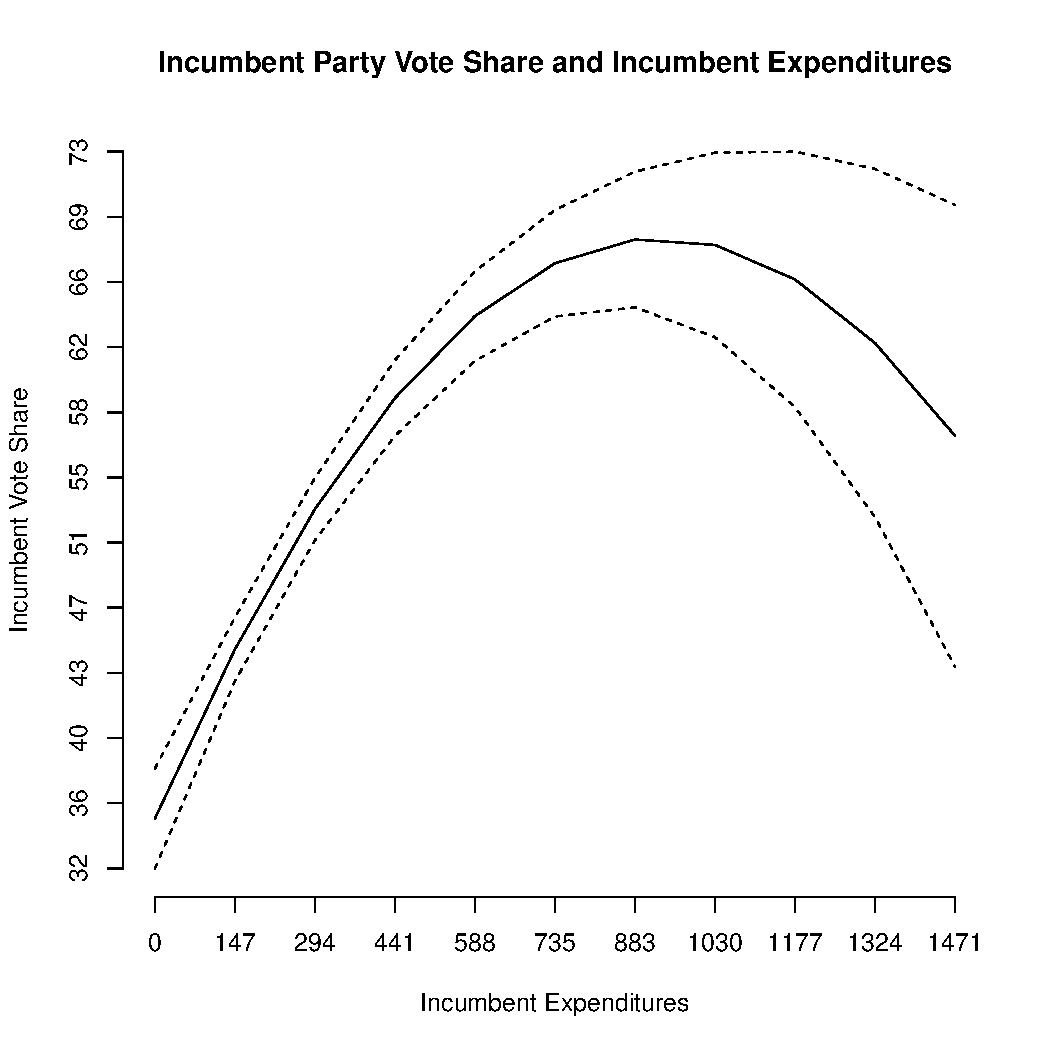
\includegraphics[width=\maxwidth]{figure/unnamed-chunk-1-1} 
\begin{kframe}\begin{alltt}
\hlcom{### c}

\hlkwd{setwd}\hlstd{(}\hlstr{"C:/Users/Jan/OneDrive/Documents/GitHub/ps630_lab/ps630_f16/"}\hlstd{)}

\hlstd{LDC} \hlkwb{=} \hlkwd{read.dta}\hlstd{(}\hlstr{"LDC_IO_replication.dta"}\hlstd{)}

\hlstd{LDC}\hlopt{$}\hlstd{regime_class} \hlkwb{=} \hlnum{NA}

\hlstd{LDC}\hlopt{$}\hlstd{regime_class[LDC}\hlopt{$}\hlstd{polityiv_update2} \hlopt{>} \hlnum{5}\hlstd{]} \hlkwb{=} \hlstr{"Democracy"}
\hlkwd{unique}\hlstd{(LDC}\hlopt{$}\hlstd{regime_class)}
\end{alltt}
\begin{verbatim}
## [1] "Democracy" NA
\end{verbatim}
\begin{alltt}
\hlstd{LDC}\hlopt{$}\hlstd{regime_class[LDC}\hlopt{$}\hlstd{polityiv_update2} \hlopt{>= -}\hlnum{5} \hlopt{&} \hlstd{LDC}\hlopt{$}\hlstd{polityiv_update2} \hlopt{<=} \hlnum{5}\hlstd{]} \hlkwb{=} \hlstr{"Anocracy"}
\hlkwd{unique}\hlstd{(LDC}\hlopt{$}\hlstd{regime_class)}
\end{alltt}
\begin{verbatim}
## [1] "Democracy" "Anocracy"  NA
\end{verbatim}
\begin{alltt}
\hlstd{LDC}\hlopt{$}\hlstd{regime_class[LDC}\hlopt{$}\hlstd{polityiv_update2} \hlopt{< -}\hlnum{5}\hlstd{]} \hlkwb{=} \hlstr{"Autocracy"}
\hlkwd{unique}\hlstd{(LDC}\hlopt{$}\hlstd{regime_class)}
\end{alltt}
\begin{verbatim}
## [1] "Democracy" "Anocracy"  "Autocracy" NA
\end{verbatim}
\end{kframe}
\end{knitrout}

Note: It is possible to take the mean values from a subset of the dataset that only contains complete cases (with values of all independent variables available). However, the effect of the Polity IV Score will not be affected by different values of the control variables because we keep those values constant in either case. Therefore, it is fine but not necessary to take the mean values from a subset with complete cases.



\pagebreak

\subsection*{Problem 2}

\begin{knitrout}
\definecolor{shadecolor}{rgb}{0.969, 0.969, 0.969}\color{fgcolor}\begin{kframe}
\begin{alltt}
\hlcom{### a}
\hlkwd{setwd}\hlstd{(}\hlstr{"C:/Users/Jan/OneDrive/Documents/GitHub/ps630_lab/ps630_f16/"}\hlstd{)}
\hlkwd{library}\hlstd{(readstata13)}
\hlstd{na_data} \hlkwb{=} \hlkwd{read.dta13}\hlstd{(}\hlstr{"na_data.dta"}\hlstd{)}
\hlkwd{summary}\hlstd{(na_data)}
\end{alltt}
\begin{verbatim}
##  countrycode             year           v_c           
##  Length:10624       Min.   :1950   Min.   :0.000e+00  
##  Class :character   1st Qu.:1973   1st Qu.:7.600e+02  
##  Mode  :character   Median :1986   Median :1.296e+04  
##                     Mean   :1985   Mean   :8.369e+06  
##                     3rd Qu.:1999   3rd Qu.:2.230e+05  
##                     Max.   :2011   Max.   :4.053e+09  
##                                    NA's   :561        
##       v_i                  v_g                 v_x           
##  Min.   :     -7427   Min.   :        0   Min.   :0.000e+00  
##  1st Qu.:       251   1st Qu.:      171   1st Qu.:4.260e+02  
##  Median :      4319   Median :     3197   Median :5.520e+03  
##  Mean   :   4418919   Mean   :  1658085   Mean   :4.787e+06  
##  3rd Qu.:     70963   3rd Qu.:    49433   3rd Qu.:8.596e+04  
##  Max.   :2433863510   Max.   :667440135   Max.   :1.955e+09  
##  NA's   :561          NA's   :561         NA's   :519        
##       v_m                v_gdp                q_c           
##  Min.   :0.000e+00   Min.   :0.000e+00   Min.   :2.000e+00  
##  1st Qu.:5.320e+02   1st Qu.:1.188e+03   1st Qu.:7.238e+03  
##  Median :6.670e+03   Median :2.077e+04   Median :1.263e+05  
##  Mean   :4.538e+06   Mean   :1.473e+07   Mean   :1.202e+07  
##  3rd Qu.:1.094e+05   3rd Qu.:3.398e+05   3rd Qu.:9.104e+05  
##  Max.   :2.194e+09   Max.   :7.427e+09   Max.   :2.343e+09  
##  NA's   :519         NA's   :519         NA's   :561        
##       q_i                  q_g                 q_x           
##  Min.   :    -39042   Min.   :        6   Min.   :0.000e+00  
##  1st Qu.:      2543   1st Qu.:     1865   1st Qu.:3.730e+03  
##  Median :     39263   Median :    27296   Median :4.116e+04  
##  Mean   :   6616470   Mean   :  2764949   Mean   :7.191e+06  
##  3rd Qu.:    279383   3rd Qu.:   224138   3rd Qu.:2.672e+05  
##  Max.   :1098261440   Max.   :372916568   Max.   :1.453e+09  
##  NA's   :561          NA's   :561         NA's   :519        
##       q_m                q_gdp                pop           
##  Min.   :7.000e+00   Min.   :9.000e+00   Min.   :4.608e+03  
##  1st Qu.:5.002e+03   1st Qu.:1.252e+04   1st Qu.:7.673e+05  
##  Median :4.708e+04   Median :2.065e+05   Median :4.951e+06  
##  Mean   :6.188e+06   Mean   :2.188e+07   Mean   :3.177e+07  
##  3rd Qu.:3.579e+05   3rd Qu.:1.424e+06   3rd Qu.:1.614e+07  
##  Max.   :1.223e+09   Max.   :3.903e+09   Max.   :1.324e+09  
##  NA's   :519         NA's   :519         NA's   :459        
##        xr                xr2               v_gfcf         
##  Min.   :    0.00   Min.   :    0.00   Min.   :0.000e+00  
##  1st Qu.:    0.90   1st Qu.:    0.91   1st Qu.:3.900e+02  
##  Median :    2.57   Median :    2.64   Median :7.822e+03  
##  Mean   :  220.40   Mean   :  221.12   Mean   :4.854e+06  
##  3rd Qu.:   28.58   3rd Qu.:   31.64   3rd Qu.:1.101e+05  
##  Max.   :31900.00   Max.   :31900.00   Max.   :2.378e+09  
##  NA's   :459        NA's   :459        NA's   :2370       
##      q_gfcf         
##  Min.   :3.000e+00  
##  1st Qu.:1.826e+03  
##  Median :4.209e+04  
##  Mean   :6.118e+06  
##  3rd Qu.:3.044e+05  
##  Max.   :1.004e+09  
##  NA's   :2390
\end{verbatim}
\begin{alltt}
\hlcom{### b}
\hlstd{na_data}\hlopt{$}\hlstd{gdpgrowth} \hlkwb{=} \hlnum{NA}
\hlkwa{for} \hlstd{(i} \hlkwa{in} \hlnum{2}\hlopt{:}\hlkwd{length}\hlstd{(na_data}\hlopt{$}\hlstd{q_gdp)) \{}
    \hlkwa{if} \hlstd{(na_data}\hlopt{$}\hlstd{countrycode[i]} \hlopt{==} \hlstd{na_data}\hlopt{$}\hlstd{countrycode[i} \hlopt{-} \hlnum{1}\hlstd{]) \{}
        \hlstd{na_data}\hlopt{$}\hlstd{gdpgrowth[i]} \hlkwb{=} \hlstd{(na_data}\hlopt{$}\hlstd{q_gdp[i]}\hlopt{/}\hlstd{na_data}\hlopt{$}\hlstd{q_gdp[i} \hlopt{-} \hlnum{1}\hlstd{]} \hlopt{-} \hlnum{1}\hlstd{)} \hlopt{*}
            \hlnum{100}
    \hlstd{\}}
\hlstd{\}}

\hlkwd{summary}\hlstd{(na_data}\hlopt{$}\hlstd{gdpgrowth)}
\end{alltt}
\begin{verbatim}
##    Min. 1st Qu.  Median    Mean 3rd Qu.    Max.    NA's 
## -66.120   1.372   4.038   3.997   6.776 205.000     728
\end{verbatim}
\begin{alltt}
\hlcom{### c}
\hlstd{na_data}\hlopt{$}\hlstd{date} \hlkwb{=} \hlstd{na_data}\hlopt{$}\hlstd{year}

\hlstd{LDC}\hlopt{$}\hlstd{countrycode} \hlkwb{=} \hlnum{NA}
\hlstd{LDC}\hlopt{$}\hlstd{countrycode[LDC}\hlopt{$}\hlstd{ctylabel} \hlopt{==} \hlstr{"Turkey"}\hlstd{]} \hlkwb{=} \hlstr{"TUR"}
\hlstd{LDC}\hlopt{$}\hlstd{countrycode[LDC}\hlopt{$}\hlstd{ctylabel} \hlopt{==} \hlstr{"SouthAfrica"}\hlstd{]} \hlkwb{=} \hlstr{"ZAF"}
\hlstd{LDC}\hlopt{$}\hlstd{countrycode[LDC}\hlopt{$}\hlstd{ctylabel} \hlopt{==} \hlstr{"Mexico"}\hlstd{]} \hlkwb{=} \hlstr{"MEX"}

\hlstd{merged_data} \hlkwb{=} \hlkwd{merge}\hlstd{(LDC, na_data,} \hlkwc{by} \hlstd{=} \hlkwd{c}\hlstd{(}\hlstr{"countrycode"}\hlstd{,} \hlstr{"date"}\hlstd{))}

\hlstd{newmodel} \hlkwb{=} \hlkwd{lm}\hlstd{(newtar} \hlopt{~} \hlstd{l1polity} \hlopt{+} \hlstd{gdpgrowth} \hlopt{+} \hlkwd{factor}\hlstd{(countrycode)} \hlopt{-} \hlnum{1}\hlstd{,} \hlkwc{data} \hlstd{= merged_data)}
\hlkwd{summary}\hlstd{(newmodel)}
\end{alltt}
\begin{verbatim}
## 
## Call:
## lm(formula = newtar ~ l1polity + gdpgrowth + factor(countrycode) - 
##     1, data = merged_data)
## 
## Residuals:
##     Min      1Q  Median      3Q     Max 
## -9.4339 -3.7056 -0.2797  4.1416 11.7623 
## 
## Coefficients:
##                        Estimate Std. Error t value Pr(>|t|)    
## l1polity                -1.4270     0.2978  -4.792 3.40e-05 ***
## gdpgrowth                0.4709     0.2907   1.620    0.115    
## factor(countrycode)MEX  15.1326     1.5137   9.997 1.63e-11 ***
## factor(countrycode)TUR  29.2080     2.7362  10.675 3.08e-12 ***
## factor(countrycode)ZAF  20.5447     2.5459   8.070 2.59e-09 ***
## ---
## Signif. codes:  0 '***' 0.001 '**' 0.01 '*' 0.05 '.' 0.1 ' ' 1
## 
## Residual standard error: 5.694 on 33 degrees of freedom
##   (52 observations deleted due to missingness)
## Multiple R-squared:  0.9176,	Adjusted R-squared:  0.9051 
## F-statistic: 73.52 on 5 and 33 DF,  p-value: < 2.2e-16
\end{verbatim}
\end{kframe}
\end{knitrout}



\subsection*{Problem 3}

\paragraph*{a)} As grader, please make sure that the person who has submitted the homework has answered all questions of this problem. This includes a brief explanation (2-3 sentences) of the student's theory and a reference to both the dependent and key independent variable.

Make sure that the students has done the following things:

\begin{enumerate}
	\item The student has explained which datasets contain the variables and provided an overview of how the variables are coded there.
	\item If and only if there were variables that were nominal or ordinal scale or coded as characters, the student has recognized that these variables have to be transformed to be used for a linear regression. Nominal variables have to be introduced as factors (dummies). Ordinal variables have to be either used as factors (dummies) or have to be assigned numerical values. Similarly, variables that are coded as characters have to be either introduced as factors (dummies) or recoded as numerical variables.
	\item The students has briefly discussed the numbers of units and the time periods covered by the datasets. Note that the discussion does not have to be extensive. (See problem set for an example)
\end{enumerate}

\paragraph*{b)} As grader, please make sure that the person who has submitted the homework has answered all questions of this problem. This includes a brief explanation of whether or not there could be measurement error in the data. If the student believes that there is no measurement error, a justification has to be given. If the student believes that there is measurement error, make sure that the students has done the following things:

\begin{enumerate}
  \item The student has explained whether there is systematic or stochastic measurement error.
  \item If the student believes that there is systematic error, the student has further elaborated on whether this bias occurs with respect to the constant or a variable, and what the specific consequences are (shifts in intercepts and descriptive stats or bias in the regression line respectively).
  \item If the student believes that there is stochastic error, the student has further elaborated on whether this bias occurs with respect to the dependent or independent variable and what the specific consequences are (higher levels of uncertainty caused by higher absolute error values and attenuation bias respectively).
\end{enumerate}

Please generally make sure that the student has described the consequences of one type of error, even if the student believes that there is no measurement error (as is asked for in the task itself).

\paragraph*{c)} As grader, please make sure that the person who has submitted the homework has answered all questions of this problem. This includes a brief theoretical explanation for the importance of at least two control variables that the student suggests to use for the final paper. For all control variables there should be a brief reference to either literature that has explained the theoretical impact of the variable, the concept of omitted variable bias, or both.

Important: when a reference to the concept of omitted variable bias is made (as the justification for the inclusion of a control variable), it is most important that the student has recognized that the \textbf{variable in question must have an influence on both the dependent and the independent variable}. Otherwise we cannot speak of the phenomenon of OVB.

Make sure that the students has done the following things:

\begin{enumerate}
	\item The student has explained which datasets contain the variables and provided an overview of how the variables are coded there.
	\item If and only if there were variables that were nominal or ordinal scale or coded as characters, the student has recognized that these variables have to be transformed to be used for a linear regression. Nominal variables have to be introduced as factors (dummies). Ordinal variables have to be either used as factors (dummies) or have to be assigned numerical values. Similarly, variables that are coded as characters have to be either introduced as factors (dummies) or recoded as numerical variables.
	\item The students has addressed potential differences (if there are any) in the time periods and units covered. For example, data for the control variables may be available only for OECD countries while the data for the dependent variable may only be available for developing countries. Another example would be that data for the control variables may be available on a quarterly basis while data for the dependent variable may be available on an annual basis.
	\item The students has addressed differences in the coding of time periods and units. For example, the names of countries may be coded as full names in one dataset while another dataset uses 3-letter isocodes to refer to countries. Another example would be that time in one dataset could be coded in the format YYYY-MM (Y = year, M = month) while it could be coded in the format YY-MM in another dataset.
\end{enumerate}

Please note that, in accordance with the task, if the student has a dataset for which no additional data can be gathered (such as individuals that were randomly selected and cannto be identified again), it is sufficient to carefully considerpotential omitted variables and how their absence might influence the results. In this case, no other datasets have to be discussed.


\section*{Statistical Theory: Omitted Variable Bias}

\subsection*{Problem 4}

\subparagraph{} Please recall that our regression was given as:

$Y = \alpha + \beta{_1}X_1 + \beta{_2}X_2 + \beta{_3}X_3 + \beta{_4}X_4 + \beta{_5}X_5 + \epsilon$

\bigskip

Where the variables represent the following concepts:

\begin{center}
  \begin{tabular}{ | l | r | }
    \hline
    $Y$ & Military Expenditures (Percent of GDP) \\ \hline
    $X_1$ & Regime Type (Polity IV) \\ \hline
    $X_2$ & External Military Threat \\ \hline
    $X_3$ & Militaristic Ideology \\ \hline
    $X_4$ & Size of the Arms Industry \\ \hline
    $X_5$ & No. of Armed Conflicts in the Last Decade\\
    \hline
  \end{tabular}
\end{center}

\bigskip

We expect that militaristic ideology is negatively correlated with democracy. Additionally, we expect that military ideology has a positive effect on military expenditures. Mathematically these statements would mean:

\bigskip

$Cov(X_1, X_3) < 0$ and $Cov(Y, X_3) > 0$

\bigskip

What would happen if we omit the variable $X_3$ from the regression? We begin with two regressions:

\begin{enumerate}
  \item $ Y = \alpha + \beta{_1}X_1 + \beta{_2}X_2 + \beta{_3}X_3 + \beta{_4}X_4 + \beta{_5}X_5 + \epsilon$
  \item $ Y = \alpha + \lambda{_1}X_1 + \beta{_2}X_2 + \beta{_4}X_4 + \beta{_5}X_5 + \epsilon{_2}$
\end{enumerate}

\bigskip

Note that the second regression has $X_3$ omitted and that we therefore expect to get a different coefficient for $X_1$, namely  $\lambda{_1}$ instead of $\beta{_1}$.

\bigskip

$\lambda{_1}$ = $\dfrac{Cov(X_1,Y)}{Var(X_1)}$.

\bigskip

Assuming that $X_3$ has some impact on $Y$, we know that $Y$ can be rewritten as a linear function of it (and the other variables that we have in the model). So:

\bigskip

$\lambda{_1}$ = $\dfrac{Cov(X_1,\alpha + \beta{_1}X_1 + \beta{_2}X_2 + \beta{_3}X_3 + \beta{_4}X_4 + \beta{_5}X_5 + \epsilon)}{Var(X_1)}$

\bigskip

We can rewrite this as:

\bigskip

$\lambda{_1}$ = $\beta{_1}*\dfrac{Var(X_1)}{Var(X_1)} + \beta{_2}*\dfrac{Cov(X_1,X_2)}{Var(X_1)} + \beta{_3}*\dfrac{Cov(X_1,X_3)}{Var(X_1)} + \beta{_4}*\dfrac{Cov(X_1,X_4)}{Var(X_1)}  + \beta{_5}*\dfrac{Cov(X_1,X_5)}{Var(X_1)} + \dfrac{Cov(X_1,\epsilon)}{Var(X_1)}$

\bigskip

Recall that the task asks you to assume that there is omitted variable bias for \textbf{one of the control variables only}. In this case, there would not be any correlation between $X_1$ and the other variables, implying that their covariances would be theoretically zero. Note that the covariance between $X_1$ and the error term is also theoretically zero if the condition holds that there is omitted variable bias for only one variable. It then follows that:

\bigskip

$\lambda{_1}$ = $\beta{_1} + \beta{_3}*\dfrac{Cov(X_1,X_3)}{Var(X_1)}$

\bigskip

Notice that the $\beta{_3} > 0$ because $Cov(Y, X_3) > 0$. However, $Cov(X_1, X_3) < 0$, meaning that:

\bigskip

$\lambda{_1}$ = $\beta{_1}$ + Positive Term $* \dfrac{Negative \ Term}{Var(X_1)}$

\bigskip

Because the variance of any variable is positive as long as there is more than one value, meaning that $Var(X_1) > 0$, the coefficient of $X_1$ would be biased downwards. 

\bigskip

Please recall that, generally, if we have the following variables:

\begin{center}
  \begin{tabular}{ | l | r | }
    \hline
    $Y$ & Dependent Variable \\ \hline
    $X_1$ & Key Independent Variable \\ \hline
    $X_2$ & Potentially Omitted Variable \\
    \hline
  \end{tabular}
\end{center}

\bigskip

The following happens if you leave $X_2$ out of the linear regression:

\bigskip

\begin{center}
    \begin{tabular}{ | l | c | r |}
    \hline
    & $Cov(X1,X2) > 0$ & $Cov(X1,X2) < 0$ \\ \hline
    $Cov(Y,X2) > 0$ & upward bias of $X_1$ coefficient & downward bias of $X_1$ coefficient \\ \hline
    $Cov(Y,X2) < 0$ & downward bias of $X_1$ coefficient & upward bias of $X_1$ coefficient \\
    \hline
    \end{tabular}
\end{center}



\end{document}
